\section*{\nr.3 \titthree (10 Punkte)}
\begin{enumerate}[(a)]
\item Es gilt $\varphi = 2\pi\frac{\Delta s}{\lambda}$ und $\Delta s = \sin{\alpha }g$. Daraus folgt
\begin{equation}
	\varphi = 2\pi\sin{\alpha}\frac{g}{\lambda}.
\end{equation}
\item Die k-te Welle hat eine Phasenverschiebung von $n\varphi$ (gezählt von 0 bis n-1). Daraus ergibt sich für die k-te Welle die komplexe Darstellung $e^{ik\varphi}$. Damit folgt
\begin{equation}
	E = E_0 \sum_{k=0}^{n-1} e^{ik\varphi} = E_0 \frac{e^{in\varphi} - 1}{e^{i\varphi}  - 1} = E_0 e^{i\frac{n-1}{2}\varphi}\frac{\sin{\frac{n}{2}\varphi}}{sin{\frac{\varphi}{2}}}.
\end{equation}
Da $|e^{i\frac{n-1}{2}\varphi}| = 1$ gilt
\begin{equation}
	I \propto |E|^2 = E_0^2 \frac{\sin^2{\frac{n}{2}\varphi}}{\sin^2{\frac{\varphi}{2}}}
\end{equation} \\
% @ Raphael, hier die Skizze, bau es ein wie es dir passt!
% @ Kianusch, danke, auch wenn du das niemals lesen wirst :P

\begin{figure}[htbp]
\centering
% GNUPLOT: LaTeX picture with Postscript
\begingroup
  \makeatletter
  \providecommand\color[2][]{%
    \GenericError{(gnuplot) \space\space\space\@spaces}{%
      Package color not loaded in conjunction with
      terminal option `colourtext'%
    }{See the gnuplot documentation for explanation.%
    }{Either use 'blacktext' in gnuplot or load the package
      color.sty in LaTeX.}%
    \renewcommand\color[2][]{}%
  }%
  \providecommand\includegraphics[2][]{%
    \GenericError{(gnuplot) \space\space\space\@spaces}{%
      Package graphicx or graphics not loaded%
    }{See the gnuplot documentation for explanation.%
    }{The gnuplot epslatex terminal needs graphicx.sty or graphics.sty.}%
    \renewcommand\includegraphics[2][]{}%
  }%
  \providecommand\rotatebox[2]{#2}%
  \@ifundefined{ifGPcolor}{%
    \newif\ifGPcolor
    \GPcolortrue
  }{}%
  \@ifundefined{ifGPblacktext}{%
    \newif\ifGPblacktext
    \GPblacktextfalse
  }{}%
  % define a \g@addto@macro without @ in the name:
  \let\gplgaddtomacro\g@addto@macro
  % define empty templates for all commands taking text:
  \gdef\gplbacktext{}%
  \gdef\gplfronttext{}%
  \makeatother
  \ifGPblacktext
    % no textcolor at all
    \def\colorrgb#1{}%
    \def\colorgray#1{}%
  \else
    % gray or color?
    \ifGPcolor
      \def\colorrgb#1{\color[rgb]{#1}}%
      \def\colorgray#1{\color[gray]{#1}}%
      \expandafter\def\csname LTw\endcsname{\color{white}}%
      \expandafter\def\csname LTb\endcsname{\color{black}}%
      \expandafter\def\csname LTa\endcsname{\color{black}}%
      \expandafter\def\csname LT0\endcsname{\color[rgb]{1,0,0}}%
      \expandafter\def\csname LT1\endcsname{\color[rgb]{0,1,0}}%
      \expandafter\def\csname LT2\endcsname{\color[rgb]{0,0,1}}%
      \expandafter\def\csname LT3\endcsname{\color[rgb]{1,0,1}}%
      \expandafter\def\csname LT4\endcsname{\color[rgb]{0,1,1}}%
      \expandafter\def\csname LT5\endcsname{\color[rgb]{1,1,0}}%
      \expandafter\def\csname LT6\endcsname{\color[rgb]{0,0,0}}%
      \expandafter\def\csname LT7\endcsname{\color[rgb]{1,0.3,0}}%
      \expandafter\def\csname LT8\endcsname{\color[rgb]{0.5,0.5,0.5}}%
    \else
      % gray
      \def\colorrgb#1{\color{black}}%
      \def\colorgray#1{\color[gray]{#1}}%
      \expandafter\def\csname LTw\endcsname{\color{white}}%
      \expandafter\def\csname LTb\endcsname{\color{black}}%
      \expandafter\def\csname LTa\endcsname{\color{black}}%
      \expandafter\def\csname LT0\endcsname{\color{black}}%
      \expandafter\def\csname LT1\endcsname{\color{black}}%
      \expandafter\def\csname LT2\endcsname{\color{black}}%
      \expandafter\def\csname LT3\endcsname{\color{black}}%
      \expandafter\def\csname LT4\endcsname{\color{black}}%
      \expandafter\def\csname LT5\endcsname{\color{black}}%
      \expandafter\def\csname LT6\endcsname{\color{black}}%
      \expandafter\def\csname LT7\endcsname{\color{black}}%
      \expandafter\def\csname LT8\endcsname{\color{black}}%
    \fi
  \fi
    \setlength{\unitlength}{0.0500bp}%
    \ifx\gptboxheight\undefined%
      \newlength{\gptboxheight}%
      \newlength{\gptboxwidth}%
      \newsavebox{\gptboxtext}%
    \fi%
    \setlength{\fboxrule}{0.5pt}%
    \setlength{\fboxsep}{1pt}%
\begin{picture}(7936.00,3968.00)%
    \gplgaddtomacro\gplbacktext{%
      \csname LTb\endcsname%
      \put(814,704){\makebox(0,0)[r]{\strut{}$0$}}%
      \put(814,1226){\makebox(0,0)[r]{\strut{}$0.2$}}%
      \put(814,1747){\makebox(0,0)[r]{\strut{}$0.4$}}%
      \put(814,2269){\makebox(0,0)[r]{\strut{}$0.6$}}%
      \put(814,2790){\makebox(0,0)[r]{\strut{}$0.8$}}%
      \put(814,3312){\makebox(0,0)[r]{\strut{}$1$}}%
      \put(1246,484){\makebox(0,0){\strut{}$-30$}}%
      \put(2245,484){\makebox(0,0){\strut{}$-20$}}%
      \put(3244,484){\makebox(0,0){\strut{}$-10$}}%
      \put(4243,484){\makebox(0,0){\strut{}$0$}}%
      \put(5241,484){\makebox(0,0){\strut{}$10$}}%
      \put(6240,484){\makebox(0,0){\strut{}$20$}}%
      \put(7239,484){\makebox(0,0){\strut{}$30$}}%
    }%
    \gplgaddtomacro\gplfronttext{%
      \csname LTb\endcsname%
      \put(176,2203){\rotatebox{-270}{\makebox(0,0){\strut{}$I/\left(I_0\cdot n^2 \right)$}}}%
      \put(4242,154){\makebox(0,0){\strut{}Ablenkwinkel $\alpha$ in $^\circ$}}%
      \csname LTb\endcsname%
      \put(3786,3530){\makebox(0,0)[r]{\strut{}$n=2$}}%
      \csname LTb\endcsname%
      \put(5169,3530){\makebox(0,0)[r]{\strut{}$n=4$}}%
      \csname LTb\endcsname%
      \put(6552,3530){\makebox(0,0)[r]{\strut{}$n=16$}}%
    }%
    \gplgaddtomacro\gplbacktext{%
      \csname LTb\endcsname%
      \put(814,704){\makebox(0,0)[r]{\strut{}$0$}}%
      \put(814,1226){\makebox(0,0)[r]{\strut{}$0.2$}}%
      \put(814,1747){\makebox(0,0)[r]{\strut{}$0.4$}}%
      \put(814,2269){\makebox(0,0)[r]{\strut{}$0.6$}}%
      \put(814,2790){\makebox(0,0)[r]{\strut{}$0.8$}}%
      \put(814,3312){\makebox(0,0)[r]{\strut{}$1$}}%
      \put(1246,484){\makebox(0,0){\strut{}$-30$}}%
      \put(2245,484){\makebox(0,0){\strut{}$-20$}}%
      \put(3244,484){\makebox(0,0){\strut{}$-10$}}%
      \put(4243,484){\makebox(0,0){\strut{}$0$}}%
      \put(5241,484){\makebox(0,0){\strut{}$10$}}%
      \put(6240,484){\makebox(0,0){\strut{}$20$}}%
      \put(7239,484){\makebox(0,0){\strut{}$30$}}%
    }%
    \gplgaddtomacro\gplfronttext{%
      \csname LTb\endcsname%
      \put(176,2203){\rotatebox{-270}{\makebox(0,0){\strut{}$I/\left(I_0\cdot n^2 \right)$}}}%
      \put(4242,154){\makebox(0,0){\strut{}Ablenkwinkel $\alpha$ in $^\circ$}}%
      \csname LTb\endcsname%
      \put(3786,3530){\makebox(0,0)[r]{\strut{}$n=2$}}%
      \csname LTb\endcsname%
      \put(5169,3530){\makebox(0,0)[r]{\strut{}$n=4$}}%
      \csname LTb\endcsname%
      \put(6552,3530){\makebox(0,0)[r]{\strut{}$n=16$}}%
    }%
    \gplbacktext
    \put(0,0){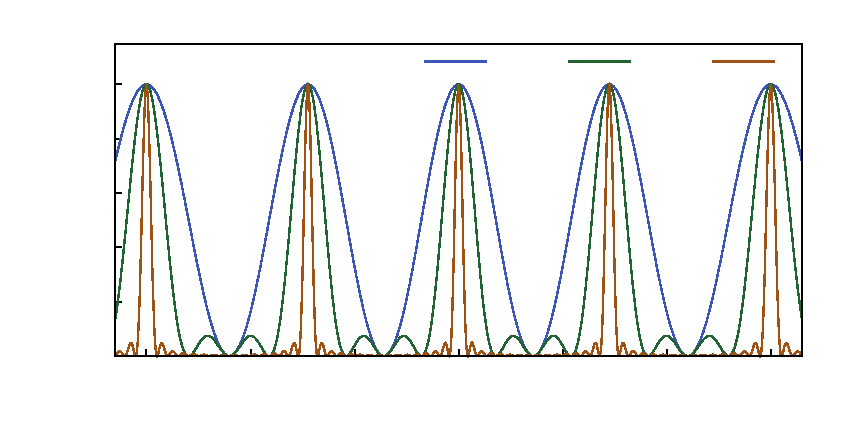
\includegraphics{beugung-Gitter}}%
    \gplfronttext
  \end{picture}%
\endgroup

\caption{Intensitätsverteilung bis zur zweiten Ordnung bei $n$ Spalten, absolut normiert und zur Vergleichbarkeit untereinander durch $n^2$ geteilt.}
\label{fig:beugung}
\end{figure}
\end{enumerate}
